\section{Experimentación}
\subsection{Introducción}
\begin{frame}
  \frametitle{Introducción}
  \begin{columns}
    \column{0.6\textwidth}
\begin{table}[!ht]
  \centering
  \scriptsize
  \begin{tabularx}{\linewidth}{|X|X|X|} \hline
\rowcolor[HTML]{FFCB2F}
\textbf{Método} & \textbf{Requisitos} & \textbf{Propósito} \\
\hline
Estimador estático de 1.75 metros. & Ninguno. & Referencia mínima.\\
\hline
Método de calibración manual. & Calibración de cámara y escena. & Referencia tradicional. \\
\hline
Método por aprendizaje profundo. & Datos de entrenamiento etiquetados & Implementación.\\
\hline
\end{tabularx}
\caption[Tabla resumen de los métodos a comparar.]{
  Tabla resumen de los métodos a comparar.
}
\end{table}
\column{0.4\textwidth}
\begin{table}[!ht]
  \scriptsize
  \centering
  \begin{tabular}{|c|c|}
    \hline
    \rowcolor[HTML]{FFCB2F}
    \textbf{Propósito} & \textbf{Dataset}\\
    \hline
    \multirow{2}{*}{Entrenamiento} & Pano360\footnotemark \\
    \cline{2-2}
                                   & COCO-Scale\footnotemark\\
    \hline
    \multirow{2}{*}{Evaluación} & KITTI-person\footnotemark\\
    \cline{2-2}
                                & IdentAI\footnotemark\\
    \hline
  \end{tabular}
  \caption{Tabla resumen de materiales.}
\end{table}
\end{columns}
\addtocounter{footnote}{-3}
\footcitetext{SPEC}
\stepcounter{footnote}
\footcitetext{SVMIW}
\stepcounter{footnote}
\footcitetext{Kitti}
\stepcounter{footnote}
\footcitetext{panacea2026}
\end{frame}

\note{
  La experimentación realizada se resumen en la siguiente tabla.
  Se realiza una comparativa entre un estimador estático que siempre predice la altura media de 1.75 metros,
  frente al método clásico y al método por aprendizaje profundo.
  El método clásico necesita intervención manual y el método por aprendizaje, una vez entrenado, es capaz
  de estimar sin referencias adicionales. El método por aprendizaje se entrena en Pano360 y COCO-Scale simultáneamente,
  y se evalua en KITTI-person e IdentAI.
}

\subsection{Método clásico}

\begin{frame}
  \frametitle{Método clásico}
  \begin{itemize}
    \item El \textbf{error absoluto medio} de los 652 fotogramas es de \textbf{6.7 centímetros}.
    \item El \textbf{error máximo} obtenido es de \textbf{41.6 centímetros}.
  \end{itemize}
  \begin{table}
    \centering
    \scriptsize
  \begin{tabular}{|l|c|c|c|c|}
  \hline
  \rowcolor[HTML]{FFCB2F}
  \textbf{Cámara} & \textbf{Soporte} & $\mu$ & $\sigma$ & \textbf{Máximo} \\
  \hline
  Cam1 & 209 & 9.2 & 7.8 & 41.6 \\
  \hline
  Cam2 & 277 & 5.2 & 3.8 & 19.4 \\
  \hline
  Cam3 & 166 & 6.2 & 3.5 & 14.9 \\
  \hline
  \textbf{Total} & \textbf{652} & \textbf{6.7} & \textbf{5.6} & \textbf{41.6} \\
  \hline
  \end{tabular}
  \caption{
  Tabla de errores de estimación del método de calibración manual en IdentAI, expresados en centímetros.
  }
  \end{table}
\end{frame}

\note{
  Aquí se puede ver los resultados del método clásico para cada cámara del conjunto IdentAI.
  Se obtiene un error medio absoluto de 6.7 centímetros y un error máximo de 41.6
  centímetros. El método manual es susceptible a acumulación de errores por imprecisión humana
  en diferentes pasos de calibración de la cámara y escena, lo que puede llevar a estas estimaciones extremas o atípicas.
}

\begin{frame}
  \frametitle{Visualización de predicciones}
\begin{figure}[!ht]
  \centering
  \subfloat{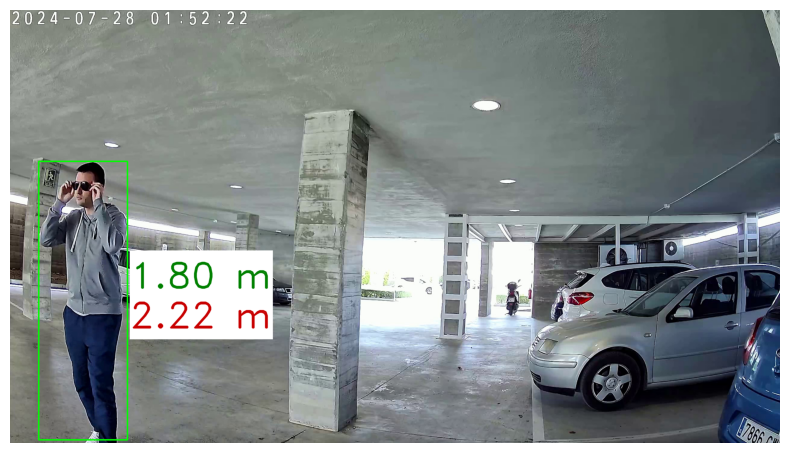
\includegraphics[width=0.5\textwidth]{imagenes/chapter4/worst_fail_cam1.png}}
  \subfloat{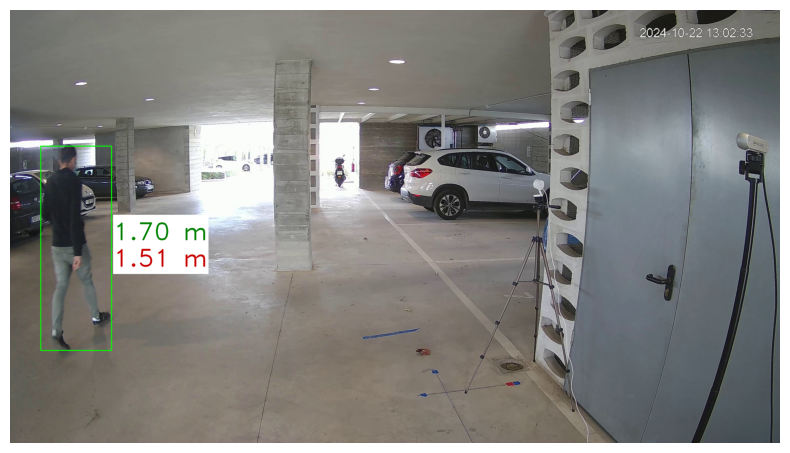
\includegraphics[width=0.5\textwidth]{imagenes/chapter4/worst_fail_cam2.png}}\\
\caption{Se observan las peores predicciones de las cámaras 1 y 2 con el método clásico.}
\end{figure}
\end{frame}

\note{
  Aquí se observan algunas de estas estimaciones atípicas.
  Los sujetos se encuentran al borde la imagen, donde las distorsiones radiales y tangenciales son
  más pronunciadas, lo que podría ser un indicativo del error de la estimación obtenida.
}

\subsection{Método por aprendizaje profundo}
\begin{frame}
  \frametitle{Método por aprendizaje profundo}
\begin{itemize}
  \item Se obtienen resultados del \textbf{mismo orden de magnitud} en Pano360\footcite{SPEC}.
  \item \textbf{CamCalib} es la implementación de Kocabas~\emph{et al.}\footnotemark[\value{footnote}] para calibración de cámara.
  \item \textbf{ScaleNet} es la implementación de Zhu~\emph{et al.}~\footcite{SVMIW}
\end{itemize}
\begin{table}[!ht]
  \centering
  \scriptsize
  \begin{tabular}{|l|c|c|c|}
  \hline
  \rowcolor[HTML]{FFCB2F}
  \textbf{Método} & \textbf{VFOV ($^\circ$)$\downarrow$} & \textbf{Pitch ($^\circ$)$\downarrow$} & \textbf{Roll ($^\circ$)$\downarrow$} \\
  \hline
  ScaleNet\footnotemark[\value{footnote}] & 5.68 & 2.61 & 1.41 \\
  \hline
  CamCalib (KL Loss)\footnotemark[\number\numexpr\value{footnote}-1\relax] & 3.53 & 2.32 & 1.15 \\
  \hline
  CamCalib (Softargmax-L2)\footnotemark[\number\numexpr\value{footnote}-1\relax] & 3.34 & 2.06 & 1.11 \\
  \hline
  CamCalib (Softargmax-biased-L2)\footnotemark[\number\numexpr\value{footnote}-1\relax] & \textbf{3.24} & \textbf{1.94} & 1.02 \\
  \hline
  \rowcolor{gray!25}
  Modelo entero fase 0 (Softargmax-biased-L2) & 3.98 & 2.43 & \textbf{0.89} \\
  \hline
  \rowcolor{gray!25}
  Solo clasificadores fase 0 (Softargmax-biased-L2) & 6.09 & 3.78 & 1.54 \\
  \hline
  \rowcolor{gray!25}
  Modelo fase final (Softargmax-biased-L2) & 3.46 & 2.34 & 1.05 \\
  \hline
  \end{tabular}
  \caption
  {
    Tabla comparativa de la precisión de la estimación de los parámetros de la cámara en Pano360\footnotemark[\number\numexpr\value{footnote}-1\relax].
}
\end{table}
\end{frame}

\note{
  Ahora; Para hablar del método por aprendizaje profundo, primero se necesita evaluar la calidad de la implementación frente al artículo de referencia.
  Por ello, se obtiene la siguiente tabla con resultados del artículo de Kocabas et al.
  En ella, se compara el rendimiento de su modelo CamCalib en la estimación de los parámetros de la cámara en las diferentes escenas de PANO360,
  en la cual se incluye ScaleNet, la implementación original de Zhu et al, y la nuestra al final de la misma.
  Los valores obtenidos son del mismo orden de magnitud y sugieren que la implementación reproduce razonablemente bien el comportamiento esperado.
  Aunque la comparación no es estrictamente directa debido a diferencias inevitables entre las particiones utilizadas (como pueden ser fotos eliminadas de la red social)
}


\begin{frame}
  \frametitle{Método por aprendizaje profundo}
  \begin{itemize}
    \item Se obtienen errores de reproyección en el \textbf{mismo orden de magnitud}.
    \item KITTI-person* consta de 1352 imágenes frente a las 298 utilizadas por Zhu~\emph{et al}~\footcite{SVMIW}.
  \end{itemize}
\begin{table}[!ht]
  \centering
  \scriptsize
  \begin{tabular}{|l|c|c|c|}
  \hline
  \rowcolor[HTML]{FFCB2F}
  \textbf{Dataset} & \textbf{Método} & \textbf{Error de reproyección} & \textbf{Error de medición}\\
  \hline
  \multirow{2}{*}{COCO-Scale} & ScaleNet SN-L3\footnotemark[\value{footnote}]& 0.07 & -\\
  \hhline{|~|-|-|-|}
                              & \cellcolor{gray!25} Nuestro & \cellcolor{gray!25} 0.07 & \cellcolor{gray!25}- \\
  \hline
  KITTI-person & ScaleNet SN-L3\footnotemark[\value{footnote}] & 0.03 & 0.10 metros\\
  \hline
  KITTI-person* & \cellcolor{gray!25}Nuestro & \cellcolor{gray!25}0.04 & \cellcolor{gray!25}0.09 metros\\
  \hline
  \end{tabular}
  \caption[Tabla comparativa de los errores de reproyección obtenidos.]{
  Tabla comparativa de los errores de reproyección y de medición obtenidos.
}
\end{table}
\end{frame}

\note{
  Respecto a la estimación de escala, comparando con una tabla obtenida del artículo de referencia de Zhu et al,
  se tiene que el error de reproyección y de estimación de altura en COCO-Scale y KITTI-person
  también están en el mismo orden magnitud. Siendo ambas cosas, otra vez, indicativos de que la implementación
  parece ser capaz replicar el comportamiento esperado.
}

\begin{frame}
  \frametitle{Método por aprendizaje profundo}
  \begin{itemize}
    \item El \textbf{error absoluto medio} a nivel de fotogramas es de \textbf{9.8 centímetros}.
  \end{itemize}
\begin{table}
  \scriptsize
  \begin{center}
    \begin{tabular}{|l|c|c|c|c|}
      \rowcolor[HTML]{FFCB2F}
      \hline
      \textbf{Dataset} & \textbf{Método} & $\mu$ & $\sigma$ & \textbf{Máximo}\\
      \hline
      \multirow{3}{*}{IdentAI}                 & Estático (1.75 metros) & 8.8 & 6.0 & 17.0 \\
      \cline{2-5}
                       & Calibración Manual & \textbf{6.7} & \textbf{5.6} & 41.6 \\
      \hhline{|~|-|-|-|-|}

                       & \cellcolor{gray!25} Nuestro & \cellcolor{gray!25} 9.8 & \cellcolor{gray!25} 6.9 & \cellcolor{gray!25} 32.8 \\
      \hline
    \end{tabular}
  \end{center}
  \caption[Tabla resumen de comparativa final en IdentAI, con errores expresados en centímetros.]{
  Tabla resumen de comparativa final en IdentAI, con errores expresados en centímetros.
  }
\end{table}
  \begin{itemize}
    \item El error absoluto medio \textbf{a nivel de sujeto} es de 7.4 centímetros.
    \item El \textbf{método clásico} presenta un error \textbf{a nivel de sujeto} de 5.8 centímetros.
  \end{itemize}
\end{frame}

\note{
  No obstante, al finalizar los experimentos y estudiar los resultados en el conjunto de datos IdentAI,
  se identifica que el modelo presenta un error absoluto medio elevado frente a los demás métodos.
  La baja variabilidad antropométrica de los datos (distribución de estatura muy centrada en 1.75 metros),
  junto a posibles problemas de aprendizaje del modelo hace que el estimador estático presente un error medio absoluto menor.
  Aún así, dichos resultados se alcanzan de forma semi-supervisada y con un bajo número de iteraciones,
  indicando el potencial que presenta el método implementado de cara a automatizar y facilitar la estimación de la altura en entornos no controlados.
}

\begin{frame}
  \frametitle{Método por aprendizaje profundo}
\begin{figure}[!ht]
  \begin{center}
    \subfloat{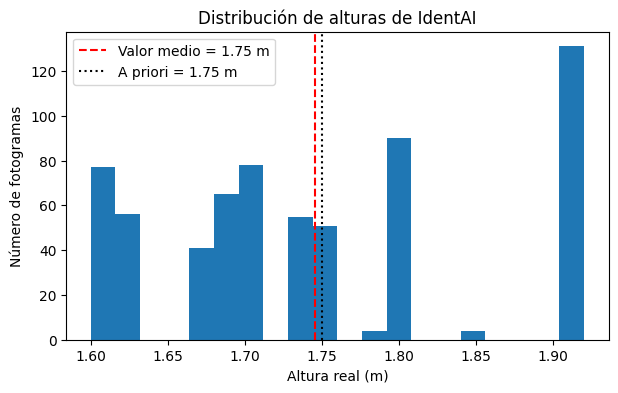
\includegraphics[width=0.5\textwidth]{imagenes/chapter4/svimw_height_dist.png}}
    \subfloat{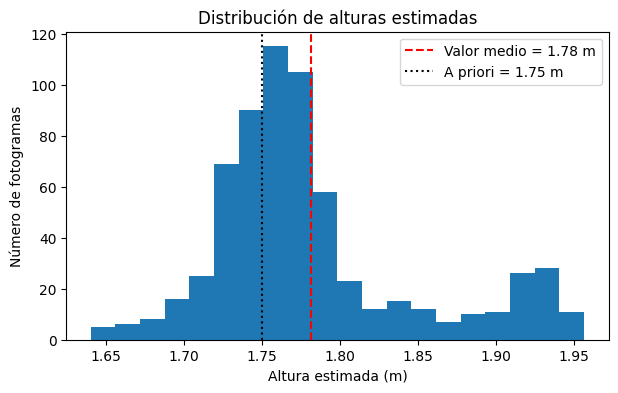
\includegraphics[width=0.5\textwidth]{imagenes/chapter4/svimw_pred_height_dist.png}}
  \end{center}
  \caption[Distribución de predicciones de altura del modelo por aprendizaje profundo.]{
  Distribución de predicciones de altura del modelo por aprendizaje profundo.
}
\end{figure}
\end{frame}

\note{
  Al estudiar las predicciones del modelo se observa un efecto de regresión hacia el a priori introducido,
  provocando que el modelo tienda a sobre-estimar para sujetos de baja estatura y subestimar para aquellos de gran estatura.
  Esto no quiere decir que el modelo no sea capaz de realizar predicciones correctas para esos extremos.
}

\begin{frame}
  \frametitle{Visualización de predicciones}
\begin{figure}[!ht]
  \centering
  \subfloat{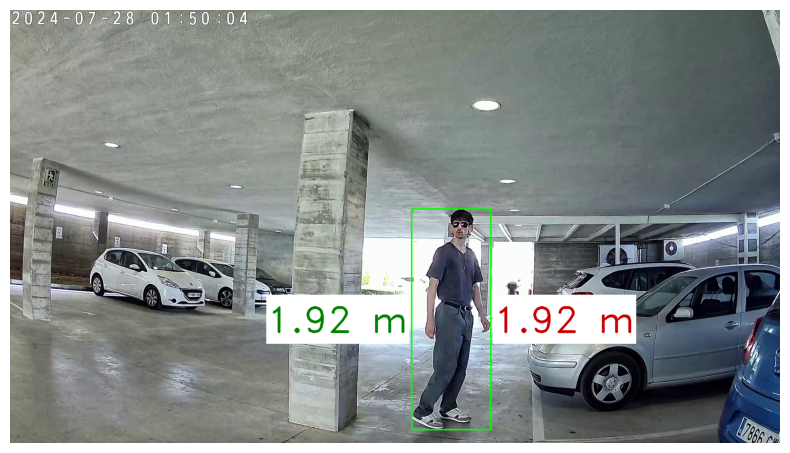
\includegraphics[width=0.5\textwidth]{imagenes/chapter4/perfect_cam1_svmiw.png}}
  \subfloat{
\includegraphics[width=0.5\textwidth]{imagenes/chapter4/perfect_cam3_svmiw.png}}\\
\caption{Se observan las mejores predicciones de las cámaras 1 y 3 con el método por aprendizaje.}
\end{figure}
\end{frame}

\note{
  En esta figura se observan predicciones coincidentes a dos decimales con valores por encima y por debajo del
  promedio de 1.75. No obstante, el efecto afecta al resultado final dado que el
  conjunto de datos presenta muchos fotogramas para el sujeto con 1.90 metros y no siempre preserva la consistencia en las predicciones
  para todos los fotogramas.
}


\begin{frame}
  \frametitle{Método por aprendizaje profundo}
  \begin{itemize}
    \item Se obtiene un \textbf{error absoluto medio} de estimación de \textbf{altura de la cámara} de 17.9 centímetros.
    \item Minimizar el error de reproyección sin suposiciones adicionales de la escena
      \textbf{no garantiza} que los \textbf{parámetros geométricos} estimados sean \textbf{físicamente correctos}.
  \end{itemize}
\begin{table}[!ht]
  \centering
  \scriptsize
\begin{tabular}{|l|c|c|c|c|}
\hline
\rowcolor[HTML]{FFCB2F}
\textbf{Cámara} & \textbf{Soporte} & $\mu$ & $\sigma$ & \textbf{Máximo} \\
\hline
Cam1 & 209 & 29.5 & 10.2 & 42.1 \\
\hline
Cam2 & 277 & 16.1 & 7.7 & 39.9 \\
\hline
Cam3 & 166 & 6.5 & 4.1 & 18.3 \\
\hline
\textbf{Total} & \textbf{652} & \textbf{17.9} & \textbf{11.8} & \textbf{42.1} \\
\hline
\end{tabular}
\caption[Tabla de errores de estimación de la altura de la cámara con aprendizaje automático, expresados en centímetros.]{
  Tabla de errores de estimación de la altura de la cámara con aprendizaje automático, expresados en centímetros.
}
\end{table}
\end{frame}

\note{
  Por último, cabe destacar el error absoluto medio de estimación de la altura de la cámara.
  Se alcanza un error medio de 17.9 centímetros.
  Esto es un indicativo que minimizar el error de reproyección de esta forma, sin suposiciones adicionales de la escena,
  no implica que las estimaciones tengan directamente sentido físico. Es decir, hay múltiples
  variaciones de altura del objeto, de la cámara y profundidad del objeto en la misma que obtienen
  el mismo bajo error de reproyección.
}
